
Calibration is a crucial procedure in the development of 
an automated robotic workcell, ensuring that all components
operate accurately and in harmony.


\begin{figure}[h]
    \centering
    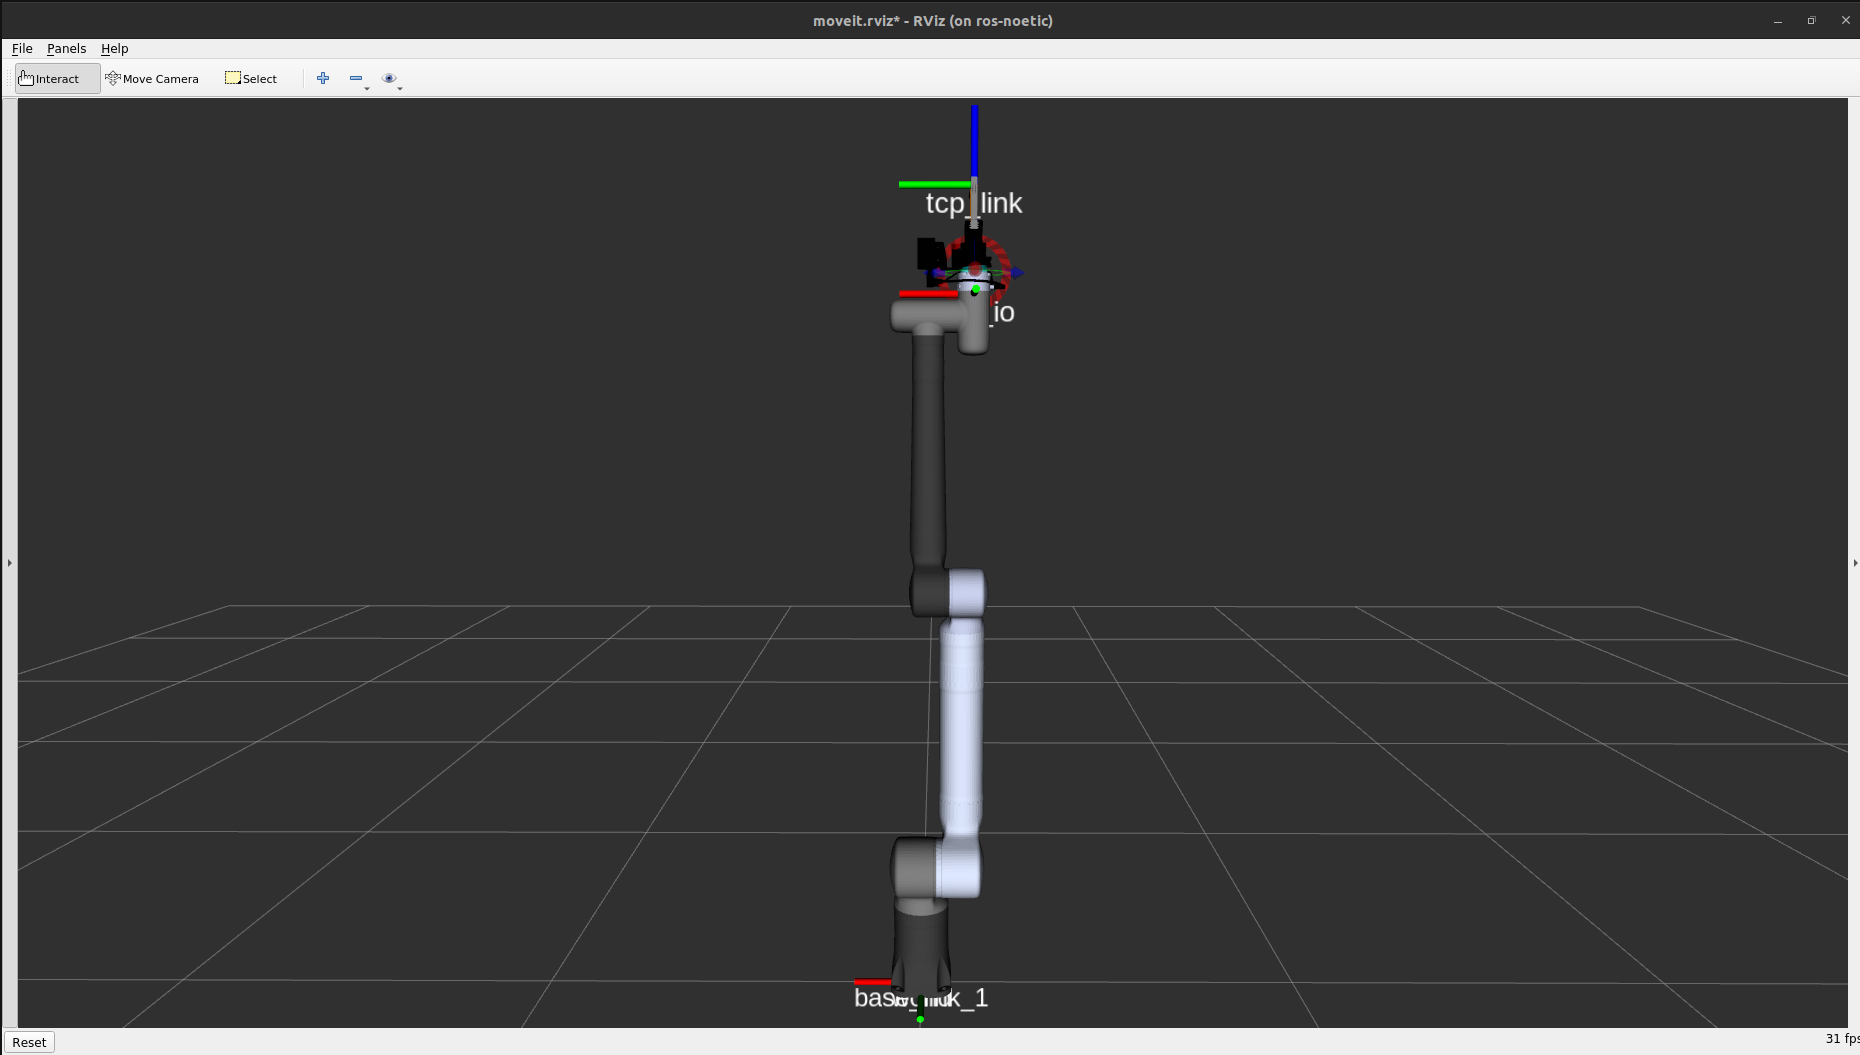
\includegraphics[width=\textwidth]{6. System Integration and Testing/6.2 Calibration Procedures/tcp.PNG}
    \caption{TCP is set at the end of gripper at a distance of 216mm from robot TOOL-IO}
    \label{fig:tcp}
\end{figure}




\subsection{Robot Calibration}
Robot calibration ensures that the Kassow robot can accurately position its end effector for loading, bending, and unloading metal sheets. This involves:

\begin{itemize}
    \item \textbf{Kinematic Calibration}: Adjusting the robot's kinematic model to correct any discrepancies between the theoretical model and the actual hardware. This includes measuring and compensating for joint offsets, link lengths, and joint angles.
    \item \textbf{Tool Center Point (TCP) Calibration}: Determining the exact position of the end effector or tool relative to the robot’s last joint. This is crucial for precise manipulation of metal sheets.
    \item \textbf{Workspace Calibration}: Defining the robot's operational workspace and ensuring that all tasks are performed within this defined area, avoiding collisions and ensuring smooth operation.
\end{itemize}

The KR1410 is already calibrated from the factory and does not need to be setup. Though in simulation, robot kinematic model is generated from the URDF and needs to be updated to match the real hardware.

\subsection{Camera Calibration}
The "Hand-Eye calibration (Robotics)" calibration method is used to determine the
reference between "Hand" (TCP) and "Eye" Camera coordinate system
(position and orientation) when the VISOR\textsuperscript{\textregistered} is attached to the gripper.
This allows different image acquisition positions and still to output the object positions
in robot coordinates directly from the camera.
\cite[page 102]{visor_user_manual}

\begin{figure}[h]
    \centering
    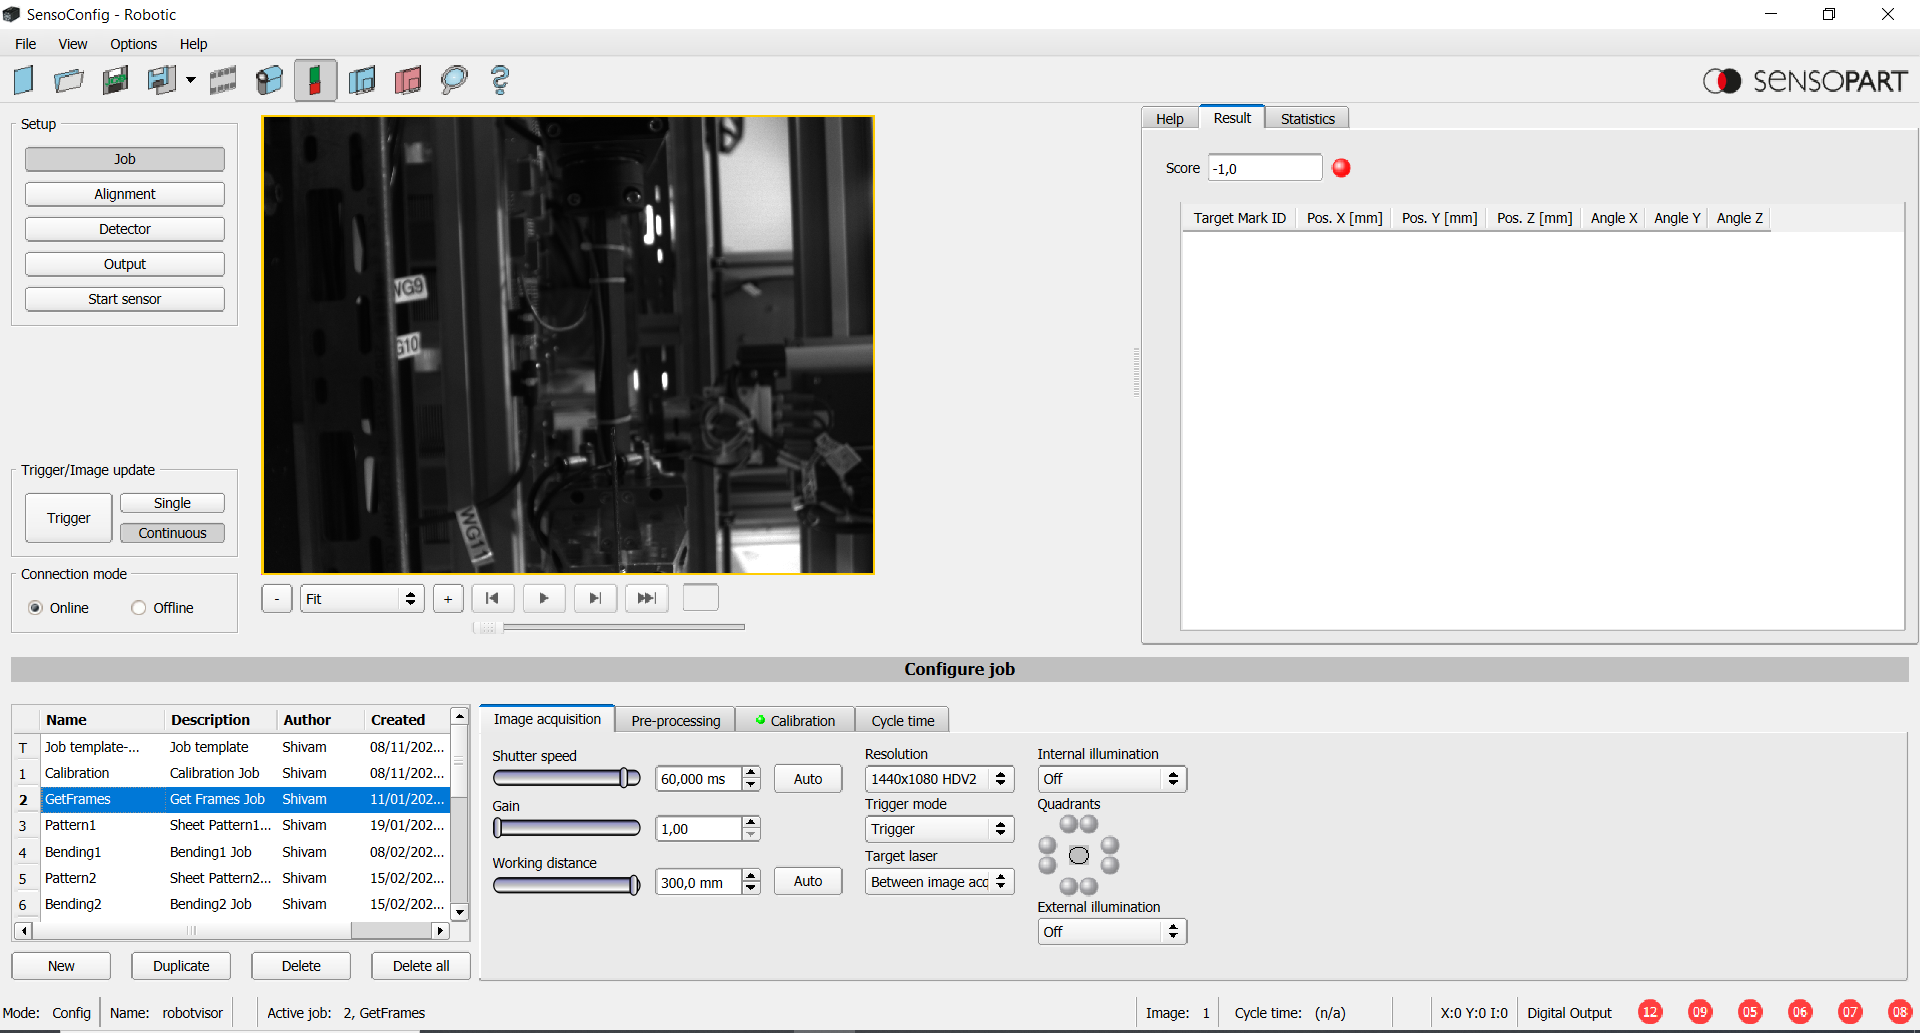
\includegraphics[width=0.9\textwidth]{6. System Integration and Testing/6.2 Calibration Procedures/shutter_speed.PNG}
    \caption{A working distance of 300mm is set for the robotic camera}
    \label{fig:working-distance}
\end{figure}

Camera calibration is essential for the accurate detection of metal sheets and measurement of bending angles. The process involves:

\begin{itemize}
    \item \textbf{Intrinsic Calibration}: Determining the camera's internal parameters, such as focal length, optical center, and lens distortion. This is typically achieved using a calibration target (e.g., a checkerboard pattern) and specialized software tools.
    \item \textbf{Extrinsic Calibration}: Establishing the camera's position and orientation relative to the robot or the workcell. This involves aligning the camera's coordinate system with the robot’s coordinate system to ensure accurate detection and measurement.
\end{itemize}

\subsection{Sensor Calibration}
Laser sensor is added to the bending machine to measure the distance between the tool and die with the reproducibility in the range of 10\textmu m. This sensor help in coordinating the bending timings between the bending machine and the robot. This sensor also requires a baseline or zero point to eliminate any offsets or biases in their readings.

\subsection{Calibration Procedures}

The calibration process is automated within the robot program
such that operator could request to re-calibrate the camera w.r.t
robot TCP from the touch panel. This allows to update the image quality as it degrades over time. 
The robot finishes the current
bending operation and then in next cycle, start with the auto-calibration.

\begin{figure}[h]
    \centering
    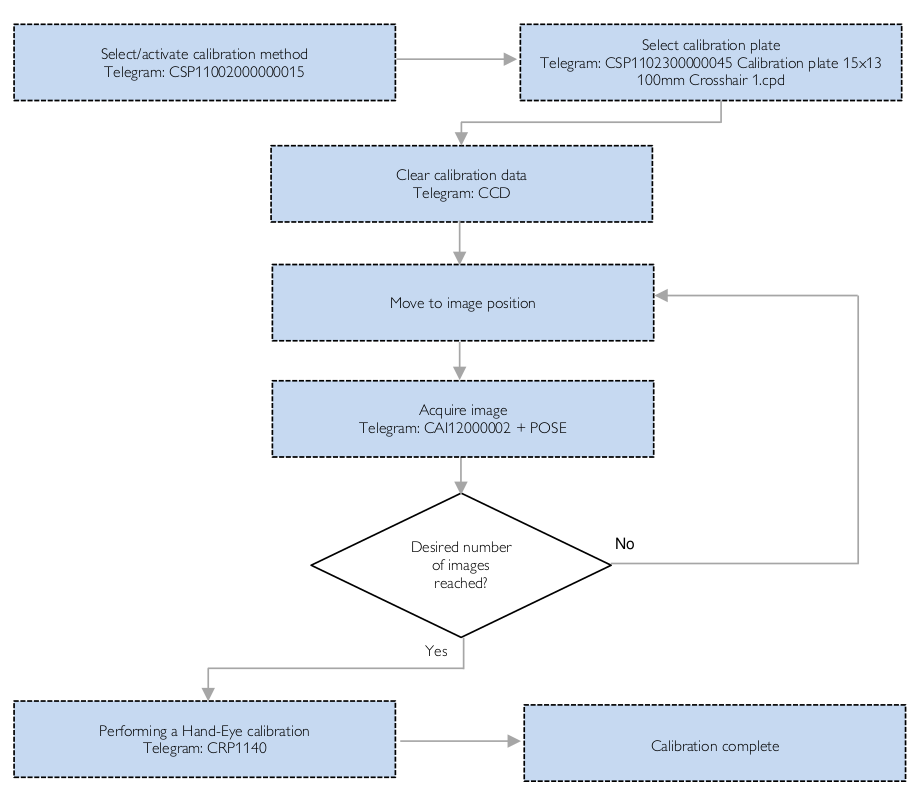
\includegraphics[width=\textwidth]{6. System Integration and Testing/6.2 Calibration Procedures/graph.png}
    \caption{Calibration procedure using telegram}
    \label{fig:calib-graph}
\end{figure}

The calibration process involves several systematic steps:

\begin{enumerate}
    \item \textbf{Setup Calibration Targets}: Place calibration targets within the robot's workspace and at specific positions that the cameras will observe.
    \item \textbf{Data Collection}: Use the robot and cameras to collect data from the calibration targets. This includes moving the robot through its range of motion and capturing images from different angles.
    \item \textbf{Parameter Estimation}: Use calibration software to estimate the parameters of the robot’s kinematic model, the intrinsic and extrinsic parameters of the cameras, and the characteristics of any other sensors.
    \item \textbf{Validation}: Verify the calibration by performing tasks that require high precision and checking the accuracy of the results. Adjust calibration parameters as needed based on validation results.
    \item \textbf{Documentation}: Record the calibration parameters and procedures for future reference and troubleshooting.
\end{enumerate}



